
% \section{Gaussian Graphical Models}

\subsection{Notation}
Let $\mathcal{S}_p$ be the set of symmetric positive definite $p \times p$ matrices. We define the vector representation of a symmetric positive definite matrix by the mapping $\text{vec} : \mathcal{S}_p \rightarrow \mathbb{R}^{p(p+1)/2}$ given by
\begin{equation*}
    \text{vec}(A) = \text{vec}\left(\begin{matrix}
        a_{1,1} & a_{2, 1} & \ldots & a_{p, 1} \\
        a_{2,1} & a_{2, 2} & \ldots & a_{p, 2} \\
                &          & \ldots & \\
        a_{p,1} & a_{p, 2} & \ldots & a_{p, p}
    \end{matrix}\right) = \left( a_{1,1}, a_{2,1}, a_{2,2}, \ldots, a_{p, p} \right)^\top, \ \forall A \in \mathcal{S}_p.
\end{equation*}

We define $\text{vec}(\mathcal{S}_p)$ to be the image of $\mathcal{S}_p$ under vec and $\text{mat} : \text{vec}(\mathcal{S}_p) \rightarrow \mathcal{S}_p$ be the inverse mapping of vec.

% Let $A \in \mathbb{R}^{p \times p}$ and $\mathcal{C} \subset \{1, \ldots, p \}$, then we define $A^{(\mathcal{C})} \in \mathbb{R}^{|\mathcal{C}| \times |\mathcal{C}|}$ as
% \begin{equation*}
%     A^{(\mathcal{C})}_{ij} = a
% \end{equation*}

\subsection{Definition}
Let $X$ be a random vector of dimension $p$ distributed according to the centered \textit{multivariate Gaussian} distribution $\mathcal{N}_p(0, \Sigma)$, where $\Sigma \in \mathcal{S}_p$ is called the \textit{covariance matrix}. The multivariate normal distribution has density function
\begin{equation*}
    f(x; \Sigma) = (2\pi)^{-p/2} |\Sigma|^{-1/2} \exp\left(-\frac{1}{2} x^\top\Sigma^{-1}x\right).
\end{equation*}
We define the \textit{precision matrix} $\Omega \in \mathcal{S}_p$ as the inverse of the covariance matrix, $\Omega = \Sigma^{-1}$. Furthermore, since $x^\top\Sigma^{-1} x \in \mathbb{R}$ and using the cyclic property of the trace, we have that $x^\top\Sigma^{-1} x = \text{tr}\left(x^\top\Sigma^{-1} x\right) = \text{tr}\left(xx^\top\Sigma^{-1}\right)$. This allows the following characterization of the density function of the multivariate normal distribution
\begin{equation} \label{eq-density-omega}
    f(x; \Omega) = (2\pi)^{-p/2} |\Omega|^{1/2} \exp\left(-\frac{1}{2} \text{tr}\left(xx^\top\Omega\right)\right),
\end{equation}

Given a random sample $X^{(1)}, \ldots, X^{(n)} \simiid \mathcal{N}_p(0, \Omega^{-1})$ we define the data matrix $X = (X^{(1)}, \ldots, X^{(n)})$, giving the log-likelihood function
\begin{equation} \label{eq-ll-omega}
    \ell(\Omega; X) = -\frac{np}{2}\log(2\pi) + \frac{n}{2}\log |\Omega| - \frac{1}{2} \text{tr}\left(XX^\top\Omega\right).
\end{equation}
For convenience, we will sometimes directly write $\ell(\Omega)$ to mean $\ell(\Omega; X)$.

\subsection{Maximum likelihood estimator of the precision matrix}

We are now interested in finding the maximum likelihood estimator of the precision matrix. To do so, we look for solutions $\hat\Omega$ to the score equation $\frac{\d}{\d\Omega}\ell(\Omega)|_{\Omega=\hat\Omega} = 0$. Using that $\frac{\partial}{\partial A_{ij}} \log|A| = A_{ij}^{-\top}$ and $\frac{\partial}{\partial A_{ij}} \text{tr}(B A) = B_{ij}^\top$ for any $A, B \in \mathbb{R}^{p \times p}$ and $i, j = 1, \ldots, p$, we can compute partial derivatives of the log-likelihood
\begin{equation*}
    \frac{\partial}{\partial\Omega_{ij}}\ell(\Omega) 
    = \frac{n}{2}\left(\Omega^{-\top}\right)_{ij} - \frac{1}{2}\left(XX^\top\right)_{ij}^\top
    = \frac{n}{2}\left(\Omega^{-1}\right)_{ij} - \frac{1}{2}\left(XX^\top\right)_{ij},
\end{equation*}
We first consider the model in which no assumptions are made on the independence relations of the components of each random vector $X^{(k)}$. In this case, the maximum likelihood estimator $\hat\Omega$ must satisfy $\frac{\partial}{\partial\Omega_{ij}}\ell(\hat\Omega) = 0$ for all $i, j = 1, \ldots, p$. Assuming that $XX^\top$ is invertible and combining the score equations yields
\begin{equation*}
    \frac{n}{2}\hat\Omega^{-1} - \frac{1}{2}XX^\top = 0 \Rightarrow \hat\Omega = \left(\frac{1}{n}XX^\top\right)^{-1}.
\end{equation*}

Note that this shows that the unconstrained maximum likelihood estimator $\hat\Omega$ is a sufficient statistic, and we can re-express the log-likelihood $\ell(\Omega; X)$ in terms of $\hat\Omega$ instead of $X$ as
\begin{equation}\label{eq-ll-mle}
    \ell(\Omega; \hat\Omega) = -\frac{np}{2}\log(2\pi) + \frac{n}{2}\log |\Omega| - \frac{n}{2} \text{tr}\left(\hat\Omega^{-1}\Omega\right),
\end{equation}
as in the first definition of the log-likelihood, we will sometimes use $\ell(\Omega)$ to mean $\ell(\Omega; \hat\Omega)$.

We now consider a second scenario in which two entries of the random vectors $X^{(k)}$ are independent, w.l.o.g.\ we assume that $X^{(k)}_1 \independent X^{(k)}_2 | X^{(k)}_3, \ldots, X^{(k)}_p$ for every $k = 1, \ldots, n$. It can be shown that this condition is equivalent to the condition $\Omega_{12} = 0$, see \cite[Proposition 5.2]{lauritzen1996}. To find the maximum likelihood estimator, we now need to solve a constrained version of likelihood equations,
\begin{align*}
    \Omega_{ij} &= 0 &&\text{for } \{i, j\} = \{ 1, 2\}\\
    \left(\Omega_{ij}\right)^{-1} &= \frac{1}{n}\left(XX^\top\right)_{ij} &&\text{otherwise}
\end{align*}
To solve this set of equations, we consider the distribution $\mathcal{N}_p(0, \Omega^{-1})$ as respecting the undirected pairwise Markov property with respect to an undirected graphical model $\mathcal{G} = (V, E)$ where the nodes $V = (1, \ldots, p)$ correspond to the coordinates of the random vector. Let $\Gamma = V \setminus \{1, 2\}$, then given that the only assumption on the independence relations of the random vector is $X^{(k)}_1 \independent X^{(k)}_2 | (X^{(k)}_3, \ldots, X^{(k)}_p)$, we have that $E = V \times \Gamma$ and hence the graph $\mathcal{G}$ contains two cliques $\mathcal{C}_1 = \Gamma \cup \{1\}$ and $\mathcal{C}_2 = \Gamma \cup \{2\}$. With this parallel made, we can rewritte the likelihood equations in terms of the cliques of $\mathcal{G}$ as
\begin{equation*}
    \left(\hat\Omega^{-1}\right)_{\mathcal{C}_i\mathcal{C}_i} = \left(XX^\top\right)_{\mathcal{C}_i\mathcal{C}_i},
\end{equation*}
for $i = 1,2$. This set of equation can be solved by \textit{Iterative proportional scaling} as described in \cite[5.2.1]{lauritzen1996}. Specializing the algorithm under the assumption $X^{(k)}_1 \independent X^{(k)}_2 | (X^{(k)}_3, \ldots, X^{(k)}_p)$, we define the marginal adjustment operators $T_i$ for $i = 1, 2$ with respectively $j = 2, 1$
\begin{align*}
    (T_{\mathcal{C}_i} \Omega)_{\mathcal{C}_i \mathcal{C}_i} &= \hat\Omega^{(\mathcal{C}_i)} + \left(\begin{matrix}
        0 & 0 \\
        0 &  \Omega_{\Gamma j} \Omega_{j \Gamma} / \Omega_{jj}
    \end{matrix}\right)\\
    (T_{\mathcal{C}_i} \Omega)_{\mathcal{C}_i^c \mathcal{C}_i^c} &= \Omega_{\mathcal{C}_i^c \mathcal{C}_i^c}
\end{align*}
where $\hat\Omega^{(\mathcal{C}_i)}$ is the unconstrained maximum likelihood operator for the subset of variables $(X_j)_{j \in \mathcal{C}_i}$. One can then show that the operator $T = T_{\mathcal{C}_2} \circ T_{\mathcal{C}_1}$ is a projection and we can thus find the maximum likelihood estimator $\hat\Omega$ from a single iteration
\begin{equation*}
    \hat\Omega = T(\mathbb{1}_p) = \left(\begin{matrix}
        \hat\Omega^{(\mathcal{C}_1)}_{11} & 0 & \hat\Omega^{(\mathcal{C}_1)}_{1 \Gamma} \\
        0 & \hat\Omega^{(\mathcal{C}_2)}_{22} &  \hat\Omega^{(\mathcal{C}_2)}_{2 \Gamma} \\
        \hat\Omega^{(\mathcal{C}_1)}_{\Gamma 1} & \hat\Omega^{(\mathcal{C}_2)}_{\Gamma 2} & \hat\Omega^{(\mathcal{C}_2)}_{\Gamma \Gamma} + \hat\Omega^{(\mathcal{C}_1)}_{\Gamma 1}\hat\Omega^{(\mathcal{C}_1)}_{1 \Gamma} /\hat\Omega^{(\mathcal{C}_1)}_{11}
    \end{matrix}\right).
\end{equation*}
Note that while $T$ is a projection, we find that $T_{\mathcal{C}_1}T \neq T$, since 
\begin{equation*}
    T_{\mathcal{C}_1}T(\mathbb{1}_p) = \left(\begin{matrix}
        \hat\Omega^{(\mathcal{C}_1)}_{11} & 0 & \hat\Omega^{(\mathcal{C}_1)}_{1 \Gamma} \\
        0 & \hat\Omega^{(\mathcal{C}_2)}_{22} &  \hat\Omega^{(\mathcal{C}_2)}_{2 \Gamma} \\
        \hat\Omega^{(\mathcal{C}_1)}_{\Gamma 1} & \hat\Omega^{(\mathcal{C}_2)}_{\Gamma 2} & \hat\Omega^{(\mathcal{C}_1)}_{\Gamma \Gamma} +  \hat\Omega^{(\mathcal{C}_2)}_{\Gamma 2}\hat\Omega^{(\mathcal{C}_2)}_{2 \Gamma} /\hat\Omega^{(\mathcal{C}_2)}_{22}
    \end{matrix}\right).
\end{equation*}

% \note{Note: we observe numerically that $\hat\Omega^{(\mathcal{C}_2)}_{\Gamma \Gamma} + \hat\Omega^{(\mathcal{C}_1)}_{\Gamma 1}\hat\Omega^{(\mathcal{C}_1)}_{1 \Gamma} /\hat\Omega^{(\mathcal{C}_1)}_{11} \approx \hat\Omega^{(\mathcal{C}_1)}_{\Gamma \Gamma} + \hat\Omega^{(\mathcal{C}_2)}_{\Gamma 2}\hat\Omega^{(\mathcal{C}_2)}_{2 \Gamma} /\hat\Omega^{(\mathcal{C}_2)}_{22}$. Could the gap be due to numerical errors? Might be true and provable equality using normality.}

\subsection{Modified likelihood root}

We start with a general presentation of the modified   likelihood root in a model with parameter $\theta = (\psi, \lambda)$ and log-likelihood $\ell$. We define the \textit{profile log-likelihod} $\ell_p$ and \textit{normalized profile log-likelihood} $\bar\ell_p(\psi)$,
\begin{align*}
    \ell_p(\psi) = \sup_{\lambda} \ell(\psi, \lambda) && \text{and} && \bar\ell_p(\psi) = \ell_p(\hat\psi) - \ell_p(\psi).
\end{align*}
Under the model assumption $\psi = \psi_0$, the the \textit{directed likelihood root} is 
\begin{equation*}
    r(\psi_0) = \text{sgn}(\hat\psi - \psi_0)\left[2 \bar\ell_p(\psi_0)\right]^{1/2}.
\end{equation*}
For fixed $p$ and under regularity conditions, the directed profile likelihood converges to a $N(0, 1)$ random variable with relative error of $O(n^{-1/2})$. This convergence will be explored in following sections. A modified version can be more accurately approximated by the standard normal, the \textit{modified likelihood root}, given by
\begin{equation}
    r^\star(\psi_0) = r(\psi_0) + r(\psi_0)^{-1}\log\left[C(\psi_0)\tilde u(\psi_0) / r(\psi_0)\right],
\end{equation}
with
\begin{align*}
    \tilde u(\psi_0) = j_p^{-1/2}(\hat\psi)\bar\ell_{p/\hat\psi}(\psi_0) && \text{and} && C(\psi_0) = |\ell_{\lambda; \hat\lambda}(\hat\theta_{\psi_0})| / \{ |j_{\lambda\lambda}(\hat\theta_{\psi_0})||j_{\lambda\lambda}(\hat\theta)| \}^{1/2}
\end{align*}

In our case, $\theta = \text{Upper}(\Omega)$ and the parameter of interest is $\psi = \Omega_{12}$ with a tested value of $\psi = \psi_0 = 0$. We can than use results from the previous sections for expressions of $\hat\Omega$ in the unconstrained case, for estimation of $\hat\theta$, and in the constrained case, for estimation of $\hat\theta_{\psi_0}$.

\begin{algorithm}\label{alg-omega-sampling}
    \SetAlgoLined
    \KwIn{Dimension $d$}
    \KwResult{Constrained precision matrix $\Omega$}

     $\Omega := 0$\;
     \While{$|\Omega| \leq 0$ }{
      Sample $\Omega \sim \mathcal{W}(\mathbb{1}_d, d)$ \;
      Set $\Omega_{12} = \Omega_{21} = 0$\;
     }
     \caption{Sampling of a precision matrix for a GGM with $X_1 \independent X_2 | X_3, \ldots, X_d$}
\end{algorithm}

\subsection{Simulations}
We implement a suite of benchmarks to analyze and compare the different test statistics for testing the hypothesis
\begin{align}\label{eq-sim-test}
    H_0: X_1 \independent X_2 | X_3, \ldots, X_d && \text{ vs. } && H_1: X_1 \notindependent X_2 | X_3, \ldots, X_d 
\end{align}
where $X \sim \mathcal{N}_d(0, \Omega^{-1})$ and the precision matrix is $\Omega \in \mathcal{S}_p$. In this setup, the quantity of interest is $\Omega$ and the number of scalar parameters to estimate is $p = d(d-1)/2$. 


We are interested in evaluating the normal approximation of $r$ and $r^\star$ under the null hypothesis (\ref{eq-sim-test}) for different scaling between the number of observations and the number of parameters, $p = O(n^\alpha)$ where $\alpha \in \{3/12, 4/12, 5/15, 6/12, 7/12, 8/12, 9/12\}$ is the scaling parameter. To do this, we fix the number of observations to $n = 1000$ and compute for each value of $\alpha$ a set of $N_p=500$ p-values for $r$ and $r^\star$ testing the hypothesis that $r$, respectively $r^\star$, is normally distributed. 

For a given value of $\alpha$, we perform $N_{\text{sim}} = 1000$ experiments to sample values of $r$ and $r^\star$ under the null hypothesis (\ref{eq-sim-test}). A Kolmgrov-Smirnov test is used to compute p-values for the null hypothesis that $r$ and $r^\star$ are respectively normally distributed.

In each experiment, we sample $n$ observations from the multivariate normal distribution $X^{(1)}, \ldots, X^{(n)} \sim \mathcal{N}_d(0, \Omega^{-1})$ with $p = n^\alpha$ and $d = p^{1/2}$. The precision matrix $\Omega$ is sampled from a Wishart distribution with $d$ degrees of freedom and the identity scaling in which the null hypothesis (\ref{eq-sim-test}) is integrated by setting $\Omega_{12} = \Omega_{21} = 0$. This is done by rejection sampling as displayed in Algorithm \ref{alg-omega-sampling}. The sample $X^{(1)}, \ldots, X^{(n)}$ is then used to compute values of $r$ and $r^\star$ according to the previous sections.

The results show that the normal approximation to the distribution of $r$ and $r^\star$ hold for every scaling parameter $\alpha$ we have tried. While the normal approximation to the $r$ statistic is expected to break for $p = O(n^{1/2})$, we do not observe this behaviour. To further explore a possible breaking point, we simulated one experiment with $n = 1000$ and $p = 990 (d = 45)$ and plotted the distribution of the p-values testing the null hypotheses $w \sim \chi^2_1$, which also seem to not expose a break behaviour.

\begin{figure}[!hbtp]
    \centering
    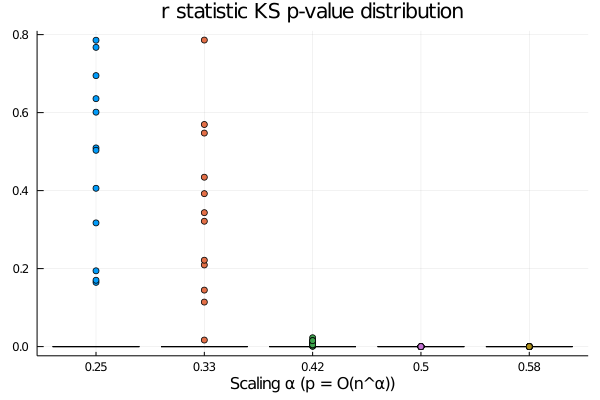
\includegraphics[scale=0.5]{r}
    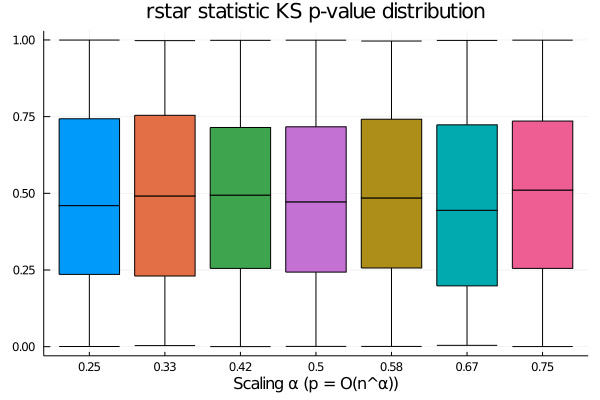
\includegraphics[scale=0.5]{rstar}
    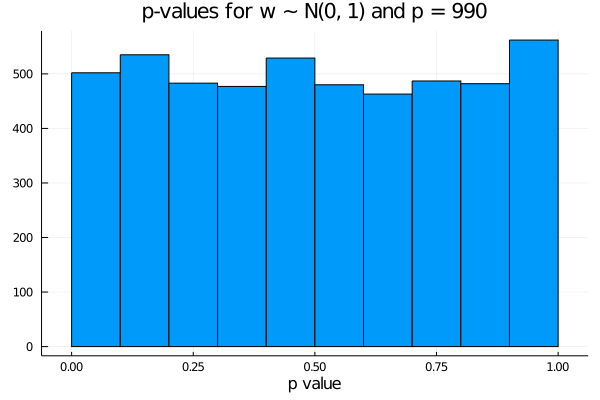
\includegraphics[scale=0.5]{w_largep}
\end{figure}

\newpage


\subsection{Multivariate normal distribution as an exponential family}
To benefit from the many existing results concerning exponential families, we reformulate the density (\ref{eq-density-omega}) as an exponential family with sufficient statistic $T$ and natural parameter $\theta \in \text{vec}(\mathcal{S}_p)$. 
\begin{equation} \label{eq-density-theta}
    f(x; \theta) = \exp\left(\theta^\top T(x) + \frac{1}{2}\log\left(|\text{mat}(\theta)|\right) - \frac{p}{2}\log\left(2\pi\right)\right),
\end{equation}
where the sufficient statistic $T : \mathbb{R}^p \rightarrow \mathcal{S}_p$ is given by $T(x) = \text{vec}(xx^t)$. Note that the canonical parameter $\theta$ is simply the vector reprensentation of the precision matrix of the multivariate normal distribution. For convenience, we use $\Omega(\theta) = (\omega_{i,j}(\theta))_{i,j}$ and $\Sigma(\theta) = (\sigma_{i,j}(\theta))_{i,j}$ to be the precision matrix and correlation matrix corresponding to the natural parameter $\theta$.

\subsection{Cumulants of the multivariate normal distributrion}

We are now interested in computing the first and second order cumulants of the multivariate normal distribution. In an exponential family with canonical parameter $\theta$ and sufficient statistic $T$, the first and second order cumulants $\kappa_i, \kappa_{i, j}$ are given by
\begin{align*}
    \kappa_i(\theta) = \mathbb{E}_\theta\left[T_i(X)\right] && \kappa_{i,j}(\theta) = \text{Cov}_\theta\left[T_i(X), T_j(X)\right].
\end{align*}

Starting with the first order cumulants, let $i \in [p(p+1)/2]$ the sufficient statistic $T$ at index $i$ is equal to $T_i(x) = x_kx_l$ for some $k \leq l$, hence
\begin{equation*}
    \kappa_i(\theta) 
    = \mathbb{E}_\theta\left[T_i(X)\right]
    = \mathbb{E}_\theta\left[X_kX_l  \right]
    = \left\{
        \begin{array}{cc}
            \text{Var}_\theta[X_k]      & \text{ if } k = l,\\
            \text{Cov}_\theta[X_k, X_l] & \text{ if } k \neq l
        \end{array}
    \right\}
    = \sigma_{k, l}(\theta).
\end{equation*}

For the second order cumulants, let $i, j \in [p(p+1)/2]$ with $T_i(x) = x_kx_l$ and $T_j(x) = x_mx_n$ for some $k \leq l$ and $m \leq n$, we then have
\begin{align*}
    \kappa_{i,j}(\theta)
    &= \text{Cov}_\theta\left[T_i(X), T_j(X)\right]\\
    &= \mathbb{E}_\theta\left[T_i(X)T_j(X)\right] - \mathbb{E}_\theta\left[T_i(X)\right]\mathbb{E}_\theta\left[T_j(X)\right]\\
    &= \mathbb{E}_\theta\left[X_kX_lX_mX_n\right] - \sigma_{k, l}(\theta)\sigma_{m, n}(\theta).
\end{align*}
By Isserlis' theorem \cite{Isserlis1918}, the fourth moment term $\mathbb{E}_\theta\left[X_kX_lX_mX_n\right]$ is
\begin{equation*}
    \mathbb{E}_\theta\left[X_kX_lX_mX_n\right] = \sigma_{k,l}(\theta)\sigma_{m,n}(\theta) + \sigma_{k,m}(\theta)\sigma_{l,n}(\theta) + \sigma_{k,n}(\theta)\sigma_{l,m}(\theta),
\end{equation*}
giving the following expressing for the second order cumulant $\kappa_{i,j}(\theta)$
\begin{equation*}
    \kappa_{i,j}(\theta) = \sigma_{k,m}(\theta)\sigma_{l,n}(\theta) + \sigma_{k,n}(\theta)\sigma_{l,m}(\theta).
\end{equation*}